\documentclass[final,1p,12pt,UTF8,review]{elsarticle}
\usepackage{ctex}
\usepackage{cite}

%% Use the option review to obtain double line spacing
%% \documentclass[authoryear,preprint,review,12pt]{elsarticle}

%% Use the options 1p,twocolumn; 3p; 3p,twocolumn; 5p; or 5p,twocolumn
%% for a journal layout:
%% \documentclass[final,1p,times,authoryear]{elsarticle}
%% \documentclass[final,1p,times,twocolumn,authoryear]{elsarticle}
%% \documentclass[final,3p,times,authoryear]{elsarticle}
%% \documentclass[final,3p,times,twocolumn,authoryear]{elsarticle}
%% \documentclass[final,5p,times,authoryear]{elsarticle}
%% \documentclass[final,5p,times,twocolumn,authoryear]{elsarticle}

%% For including figures, graphicx.sty has been loaded in
%% elsarticle.cls. If you prefer to use the old commands
%% please give \usepackage{epsfig}
\usepackage{amssymb}
\usepackage{amsthm}
\usepackage{lineno}
\usepackage{listings}
\usepackage{color}
\usepackage{xcolor}
\usepackage{geometry}
\usepackage{amsmath}
\usepackage{booktabs}
\usepackage{graphicx}
\usepackage{float}
\usepackage{url}
\usepackage{algorithmic}
\usepackage{algorithm}
\usepackage{graphicx}
\usepackage{textcomp}
\usepackage{mathrsfs}

\definecolor{dkgreen}{rgb}{0,0.6,0}
\definecolor{gray}{rgb}{0.5,0.5,0.5}
\definecolor{mauve}{rgb}{0.58,0,0.82}

\lstset{
  language=sh,
  basicstyle=\ttfamily,
  numbers=left,
  numberstyle=\tiny,
  numbersep=5pt,
  tabsize=2,
  extendedchars=true,
  breaklines=true,
  keywordstyle=\color{purple},
  frame=shadowbox,
  stringstyle=\color{red},
  commentstyle=\color{green},
  showspaces=false,
  showtabs=false,
  xleftmargin=17pt,
  framexleftmargin=17pt,
  framexrightmargin=5pt,
  framexbottommargin=4pt,
  showstringspaces=false,
  morekeywords={},
  emph={docker,apt},
  emphstyle=\color{blue}
}


\journal{Deep Learning Course Final Report}

\begin{document}

\begin{frontmatter}

\title{基于Swin Transformer的深度强化学习方法}

\author[a]{于海龙}
\affiliation[a]{organization={南开大学\enspace 软件学院},
            postcode={2120220695}}

\author[b]{刘方圆}
\affiliation[b]{organization={南开大学\enspace 软件学院},
            postcode={2120220707}}

\begin{abstract}
\par
在深度学习领域内,模型大小的增加显著提高了模型准确率。 Transformer 在自然语言处理领域展示出了优秀的效果,在视觉任务中也逐步发展出了 Swin Transformer 模型。模型规模的增加也对计算机提出了更高的算力要求,分布式计算是一种有效的方法解决这个问题,而对数据预处理和模型进行改进也是一种有效的方法。这里使用 Double Deep Q-Learning 的方法结合 Swin Transformer 实现了一种在线强化学习方法,完成 Atari 游戏的训练。

\end{abstract}

%%Graphical abstract
% \begin{graphicalabstract}
%\includegraphics{grabs}
% \end{graphicalabstract}

% %%Research highlights
% \begin{highlights}
% \item Research highlight 1
% \item Research highlight 2
% \end{highlights}

\begin{keyword}
%% keywords here, in the form: keyword \sep keyword
Reinforement Learning \sep Deep Learning \sep Transformer

\end{keyword}

\end{frontmatter}
% \linenumbers
\newpage
\tableofcontents
\newpage
%% main text
\section{Introduction}
\par
深度神经网络是机器学习领域的一种网络模型。近年来深度学习取得了可观的发展,在计算机视觉、语音识别和自然语言处理 (Natural Language Processing, NLP) 等领域均被广泛应用。深度学习 (Deep Learing, DL) 的结构一般是含多个隐藏层的多层感知器。数据集容纳了更庞大的样本数量和计算机算力的提高帮助深度学习取得了不错的效果,数据集训练数据的增加降低了方差,而计算机算力的提高则允许深度学习训练更大规模的神经网络模型,降低偏差。% \cite{fan}
深度学习模型规模的增加提供了很好的模型精确度增益,例如在自然语言处理领域内广泛使用的 Transformer 模型。% \cite{vaswani}
\par
另一方面,强化学习 (Reinforcement Learning, RL) 被认为是人工智能的子领域,可以使用神经网络处理时间序列。目前最先进的强化学习解决方案依赖于马尔可夫决策过程 (Markov Decision Process, MDP) 来构建时间决策模型,这个模型描述了一个离散时间随机控制过程,可以通过动态规划进行数学求解。

\par
Transformer 是目前解决 NLP 任务的常用方案,在引入 Transformer 之前,处理 NLP 任务最常见的深度学习解决方案是利用递归神经网络 (Recurrent Neural Networks, RNN) 。RNN 接受可变长度的输入,并使用内部状态依次处理 token 。长短期记忆 (Long Short Term Memory, LSTM) 神经网络通过门控机制解决RNN中梯度消失或爆炸的问题,而注意力机制可以解决RNN中的长期依赖困境。Soft attention 只关注预测下一个单词的相关输入,误差可以传播到网络中产生隐藏状态的相关部分,但只有最后一个隐藏状态能够与它自己基于注意力的上下文向量一起表示。Transformer 使用 self-attention 网络,使用基于注意力的上下文向量对每个隐藏状态进行编码,当堆叠在多个 NN 层上时,会产生更丰富的上下文表示,也不受顺序严格的限制。此外Transformer 使用位置嵌入对输入标记的相对位置进行编码。

\par
在计算机视觉 (Computer Vision, CV) 领域 Transformer 也有很好的表现,如Vision Transformer (ViT) 和 Swin Transformer 。将 Transformer 应用在 CV 领域存在一些困难,因为输入数据存在尺寸比例等可变属性,但同时也避免了 NLP 任务中序列长期依赖的问题,并且可以展示图像中远距离像素之间或像素与实体之间远程依赖关系的强度。

\par
强化学习研究环境中的行为,这些环境通常要求智能体最大化其获得的奖励。在强化学习过程中,智能体通过与环境的交互来学习并改进其决策策略。其中,探索是指智能体主动尝试新的行动,以了解环境并发现可能的奖励;利用是指基于已知信息选择已知最优的行动,以最大化累积奖励。如果智能体过于探索,会花费大量时间和资源在探索新行动上,可能无法获得足够的累积奖励;如果智能体过度利用,可能会陷入一种局限的行动模式,无法发现更好的行动选择。

\par
Q-Learning 是一种基于值函数的经典的强化学习算法,用于解决基于马尔可夫决策过程的环境中的问题,通过学习最优行动值函数来指导智能体的决策,这种方法的 Q 值根据 Bellman 最优方程\ref{eq:qlearning}更新策略。$Q^*(s,a)$表示在状态$s$下采取动作$a$的最优Q值,代表在当前状态下采取特定动作的长期回报期望。$r_{t+1}$表示在$t+1$时刻的即时奖励,即在状态$s$下采取动作$a$后获得的奖励信号。$\gamma$表示折扣因子,是一个在0和1之间的值,用于衡量当前奖励和未来奖励的重要性,决定智能体对未来奖励的重视程度。

\begin{figure}[htp]
    \begin{equation}
        \label{eq:qlearning}
        Q^*(s,a)=E\{r_{t+1}+\gamma \max_{a'}Q^*(s_{t+1},a^{'}| s_t=t, a_t=t)\}
    \end{equation}
\end{figure}
% \label{eq:qlearning}
% \[Q^*(s,a)=E\{r_{t+1}+\gamma \max_{a'}Q^*(s_{t+1},a^{'}| s_t=t, a_t=t)\}\]

\par
强化学习算法可以分为 on-policy 和 off-policy 算法。on-policy 算法在同一策略上操作和更新,off-policy算法在不同策略上操作和更新。Q-learning 是 off-policy 的,因为它在$s_(t+1)$处被允许做出不同于$\max$选择的贪婪行动。将强化学习策略与神经网络相结合也成为强化学习中普遍的做法, CNN 已经被大量应用于深度强化学习任务中带有图像显示的游戏。

\par
Deep Q-learning Network (DQN) 是一种强化学习方法,它将 Q 值存储在神经网络中,并产生 Q 值预测作为网络输出。 DQN 在许多雅达利 (atari) 游戏中达到了人类或超人的水平。已有研究将 ViT 用于图像像素的强化学习,由于相对于输入图像大小的二次复杂度,在强化学习中训练 ViT 是非常昂贵的,因此大规模训练是不现实的。带 Swin Transformers 的在线强化学习方案 Swin DQN 可以将广为采用的 Double Q-learning 扩展到最近引入的 Swin Transformers 。该方法的核心是将图像像素组拆分为小的标记化补丁,并在固定大小的移位窗口内应用局部自注意力操作作为扩展。

\section{Related Work}
% \subsection{Decision Transformer}
Decision Transformer 将强化学习问题视为与 NLP 相同的序列建模问题,用因果屏蔽变压器 (Causal Masking Transformer) 代替深度学习中传统的价值函数和策略梯度方法。Decision Transformer 的一个主要限制是它只适用于离线强化学习。在训练模型之前,必须知道状态、动作和回报。Online decision transformer (ODT) 通过在统一框架中集成离线预训练和在线微调来解决这个问题,并在 D4RL 基准上实现了最先进的性能。
\section{Methodology}
% \subsection{Double Q-Learning}

\begin{figure}[htp]
    \begin{equation}
        \label{eq:dqa}
        Q^A(s,a)=Q^A(s,a)+\alpha(s, a)(r+\gamma Q^B(s^{'},a^*)-Q^A(s,a))
    \end{equation}
\end{figure}

\begin{figure}[htp]
    \begin{equation}
        \label{eq:dqb}
        Q^B (s,a) = Q^B (s,a) + \alpha(s, a)(r+\gamma Q^A(s^{'},a^*)-Q^B(s,a))
    \end{equation}
\end{figure}

\begin{algorithm}[htp]
    \caption{\label{DQN}Double Q-Learing}
    \begin{algorithmic}[1]
        \STATE \textbf{Input:} $\epsilon, \gamma, maxFrames, syncFrames, L()$
        \STATE \textbf{Parameter:} $D, Q_\theta^A, Q_\theta^B$
        \STATE \textbf{Output:} $Q_\theta^A$
        \STATE $frames \gets 0$
        \WHILE{$frames < maxFrames$}
        \STATE 初始化
        \WHILE{游戏尚未完成}
        \IF{$random()<\epsilon$}
        \STATE 随机选择行动
        \ELSE
        \STATE 从$Q_\theta^A$中选择行动
        \ENDIF
        \STATE 将$s,a,s^{'},r,terminal$存储至经验回放缓存$D$
        \STATE 从缓存$D$中抽取小批量样本进行训练
        \STATE 按照算法\ref{NetworkUpdate}更新$Q_\theta^A$
        \ENDWHILE
        \IF{$frames \% syncFrames == 0$}
        \STATE $Q_\theta^B \gets Q_\theta^A$
        \ENDIF
        \ENDWHILE
    \end{algorithmic}
\end{algorithm}

\par
Double Q-learning 是一种用于增强学习的算法,用于解决传统 Q-learning 中存在的估计偏差问题。在传统的 Q-learning 算法中,使用一个 Q 函数来估计每个状态动作对的价值,但是由于使用同一个 Q 函数进行估计和选择动作,可能会导致估计值的偏差,进而影响决策的质量,会倾向于高估 Q 值,因为策略更新了由$\max$算子选择的目标值,这使高估方向上的近似估计误差持续存在。Double Q-learning 通过使用两个独立的 Q 函数,来减少估计偏差,将动作选择和值函数更新分开进行,使用一个 Q 函数\ref{eq:dqa}来选择动作,并使用另一个 Q 函数\ref{eq:dqb}来评估选择的动作的价值,其中$Q^A$为策略网络,$Q^B$为目标网络。这种方式使得 Q 函数的选择和评估是独立的,可以减轻传统 Q-learning 中估计偏差的问题。通过交替地使用两个 Q 函数进行动作选择和值函数更新, Double Q-learning 可以减少估计偏差,提高学习的效果,在一些问题上表现出更好的性能和稳定性。实现 Double Q-learning 的惯例是保留目标 Q 网络的副本,与维护两个不同的网络相比减少了计算开销。同时需要在一定的步数之后同步策略网络和目标网络,这也是一个需要调优的超参数。 Double Q-Learning 的执行过程如算法\ref{DQN}所示,其中$\gamma$是折扣因子,$\epsilon$是探索比,$maxFrames$是最大总帧数,$L()$是损失函数,$syncFrames$是两个网络同步之间的帧数,$s$代表当前状态,$s^{'}$代表下一个状态,$a$代表行动,$r$代表奖励,而$terminal$表示游戏是否结束。在算法\ref{NetworkUpdate}中,$a^*$代表$\arg\max_aQ_\theta^A(s^{'},a)$。

\begin{algorithm}[htp]
    \caption{\label{NetworkUpdate}Network Update}
    \begin{algorithmic}[1]
        \STATE \textbf{Input:} $s,a,s^{'},r,terminal, L()$
        \STATE \textbf{Parameter:} $D, Q_\theta^A, Q_\theta^B$
        \STATE \textbf{Output:}
        \STATE $target = r + \gamma Q_\theta^B(s^{'},a^*)*(1-terminal)$
        \STATE $loss = L(Q_\theta^A(s,a), target)$
        \STATE 使用梯度下降法更新$Q_\theta^A$
        \RETURN
    \end{algorithmic}
\end{algorithm}

\par
注意力机制在 Transformer 中被广泛应用,用于捕捉输入序列中不同位置之间的关联性,从而实现对序列的建模和表示学习。如公式\ref{eq:attention}实现为查询$Q$、键$K$和值$V$的上下文嵌入,$B$是从绝对位置嵌入改进的相对位置偏差,$d_k$是$Q$和$K$的维度。
\begin{figure}[htp]
    \begin{equation}
        \label{eq:attention}
        Attention(Q,K,V) = Softmax\left(\frac{QK^T}{\sqrt{d_k}}+B\right)V
    \end{equation}
\end{figure}

\par
这里使用 Swin Transformers 的自适应取代 CNN ,  Swin MLP 实现了多头自注意力机制作为分组1D卷积,在图像输入上仅使用一层二维卷积产生初始空间嵌入。图像像素被分割为小块并转置,使输出通道成为隐藏嵌入。通过分组的1D卷积层在自注意力机制之前完成补丁分组到局部窗口的操作。当窗口大小固定时,这种局部性的利用将计算复杂度从二次型降低到线性型。在这之后是两个线性层,其中隐藏单元的数量与嵌入维度成正比,然后是反转窗口分区的重塑操作。

\begin{figure}[htp]
    \begin{equation}
        \label{eq:GeLU_math}
        GeLU(x) = xP(X<=x)=x\Phi(x)
    \end{equation}
\end{figure}

\par
这里选择高斯误差线性单元 (Gaussian Error Linear Unit, GeLU) 代替 ReLU 作为激活函数,其数学表达如公式\ref{eq:GeLU_math}所示, GeLU 算法的简化计算如公式\ref{eq:GeLU}所示,具有更平滑的非线性特征,在自然语言处理和计算机视觉领域可以提高模型的性能。与 ReLU 对比, GeLU 在处理负数时不会像 ReLU 一样将输入裁剪到0,这可能导致梯度消失的问题。
\begin{figure}[htp]
    \begin{equation}
        \label{eq:GeLU}
        GeLU(x) = 0.5 * x * (1 + \tanh(\sqrt{\frac{2}{\pi}} * (x + 0.044715 * x^3)))
    \end{equation}
\end{figure}

\par
这里选择 Dropout 方法解决梯度下降过程中的过饱和问题。Dropout 方法的随机丢弃操作有助于减少特定神经元的过度依赖,从而鼓励网络中更多的神经元参与训练过程。通过随机丢弃部分神经元,可以减少权重的过度学习,使得网络的学习过程更加平滑,从而减轻过饱和问题的影响。除此之外, Dropout 方法还有正则化效果,可以减少过拟合并增加网络的泛化能力。

\section{Experiments}
实验在 Arcade Learning Environment (ALE) 的 Atari 游戏中进行。这里根据表\ref{DDQN}和表\ref{SDQN}设置参数,并以bowling游戏为目标进行训练,训练结果如图\ref{bowling}所示。可以看到 Swin DQN 的表现比 Double DQN 有一定程度的提高,但由于训练时间不足,尚未完成后续训练。
\begin{table}[http]
    \centering
    \caption{Double DQN 参数}
    \label{DDQN}
    \begin{tabular}{c||c}
      \hline\hline
      输入 & $84\times 84\times 4$ \\
      \hline
      优化器 & Adam \\
      \hline
      学习率 & $0.0000625$ \\
      \hline
      $\gamma$ & $0.99$ \\
      \hline
      初始$\epsilon$ & $1$ \\
      \hline
      最终$\epsilon$ & $0.01$ \\
      \hline
      $\epsilon$衰变 & $100000$ \\
      \hline
      $syncFrames$ & $40000$ \\
      \hline
      每步$Frames$ & $4$ \\
      \hline
      每步更新 & $4$ \\
      \hline
      评估步数 & $250000$ \\
      \hline
      经验回放 & $100000$ \\
      \hline
      Batch Size & $32$ \\
      \hline\hline
    \end{tabular}
\end{table}
\begin{table}[http]
    \centering
    \caption{Swin DQN 参数}
    \label{SDQN}
    \begin{tabular}{c||c}
      \hline\hline
      层 & $3$ \\
      \hline
      每层的块 & $2,3,2$ \\
      \hline
      每层的头 & $3,3,6$ \\
      \hline
      Batch Size & $3 \times 3$ \\
      \hline
      窗口大小 & $7 \times 7$ \\
      \hline
      向量维度 & $96$ \\
      \hline
      多层感知机宽深比 & $4$ \\
      \hline
      Dropout率 & $0.1$ \\
      \hline\hline
    \end{tabular}
\end{table}

\begin{figure}[htp]
    \centerline{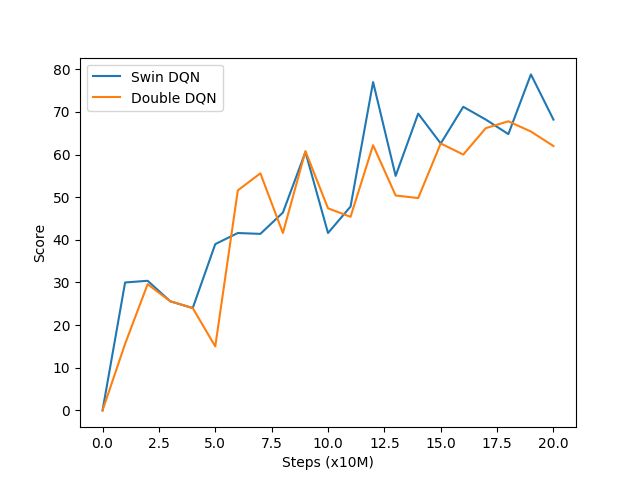
\includegraphics[width=8.5cm]{result.png}}
    \caption{Bowling Game Training Result\label{bowling}}
\end{figure}

\section{Conclusion}
在 Atari 游戏中, Swin Transformers 可以提高 DQN 的性能。空间自注意力机制 (Spatial self-attentions) 有利于普通的计算机视觉任务和基于图像的强化学习任务。与 Decision transformer 相比, Swin DQN 是一种可行且有效的方法,通过引入空间自注意力机制提高深度强化学习模型性能。

% \newpage
% \bibliographystyle{elsarticle-num} 
% \bibliography{reference}

% \begin{thebibliography}{00}

%% \bibitem[Author(year)]{label}
%% Text of bibliographic item

% \bibitem[ ()]{}

% \end{thebibliography}
\newpage
\appendix
\section{研究方向}
于海龙主要研究方向为区块链,目前面临的问题为分布式系统数据同步过程通信瓶颈,负责完成环境配置、代码编写和运行与检查和文章报告撰写。刘方圆主要研究方向为强化学习,负责完成代码编写和文章报告检查。实际工作量为各50\%。
\section{课题选择}
以强化学习方向为基础,选择深度强化学习的目标是希望使用深度学习实现一个可以根据音频乐谱序列输入输出合理演奏指法的智能体。但由于这种实验目标需要自行设计指法评分并且训练过程可预期的需要消耗大量时间,在这个过程中选择复现 Deep Reinforcement Learning with Swin Transformers 文章的方法,受设备算力限制,仅完成游戏 bowling.bin 的复现。
\section{运行环境}
\subsection{Docker}
\begin{lstlisting}[language=sh]
    docker run -itd -v "D:\Projects\DLHW:/rl" --gpus "device=0" --name "DLHW" ubuntu /bin/bash
\end{lstlisting}
在docker容器内执行`python3 /DLHW/run.py -c'
\subsection{Linux}
\begin{lstlisting}[language=sh]
    apt install python3 pip cmake zlib1g-dev git libsdl1.2-dev -y
    pip install -r requirements.txt
\end{lstlisting}
\subsection{Python requirements.txt}
\begin{lstlisting}
numpy==1.23.4
IPython
touch
opencv_python
matplotlib
timm
scipy
imageio
atari_py
\end{lstlisting}
\subsection{GitHub Repo}
\url{https://github.com/EternallyAscend/DLHW}

\end{document}

\endinput
%%
%% End of file `elsarticle-template-harv.tex'.
